\documentclass[12pt]{article}
\usepackage{../../preamble2}

\newcommand{\modulo}[1]{~(\mathrm{mod}~#1)}
%\newcommand{\modulo}[1]{~\%#1}

\newcolumntype{C}{>{$}c<{$}}% \usepackage{array}

\title{UCLA Math Circle}
\author{James Toche (and family)}
\date{19 June 2020 \\(Last revision: \today)}

\begin{document}
\begin{minipage}{\textwidth}
\maketitle
\begin{abstract}
Notes on modular arithmetic from the UCLA Math Circle Intermediate-2 for Summer Session 2020, July 19th. 
\end{abstract}
\end{minipage}

\newpage
\section*{1.2}
\begin{question}
If $a\equiv b\modulo{m}$, then $(a+m)\equiv b\modulo{m}$
\end{question}

Let $\modulo{m}$ denote ``modulo $m$''.  The first statement is equivalent to: 
\begin{align*}
a\equiv b\modulo{m}
 & \iff
\exists k\in\mathbb{N}: a = km + b
\end{align*}
where $b$ is the remainder of the division of $a$ by the modulus $m$. 

The second statement is equivalent to: 
\begin{align*}
(a+m)\equiv b\modulo{m}
 & \iff
\exists l\in\mathbb{N}: a+m = lm + b
\end{align*}

Proof: $\exists k\in\mathbb{N}$:
\begin{align*}
a 
  & = km + b \\
a + m
  & = km + b + m \\
a + m 
  & = (k+1)m + b
\end{align*}
We set $l=k+1$, where $l\in\mathbb{N}$ since $k$ and $1$ are in $\mathbb{N}$.$\qed$


\clearpage
\section*{2.1}
\begin{question}
If $a\equiv b\modulo{m}$ and $b\equiv c\modulo{m}$, then $a\equiv c\modulo{m}$.
\end{question}

The starting point is:
\begin{align*}
\exists k\in\mathbb{N}: a & = km + b \\
\exists l\in\mathbb{N}: b & = lm + c 
\end{align*}
for $a,b,c$ in $\mathbb{N}$. By simple substitution,
\begin{align*}
a & = km + b \\
  & = km + lm + c \\
  & = (k+l)m + c 
\end{align*}
where $(k+l)\in\mathbb{N}$ since $k\in\mathbb{N}$ and $l\in\mathbb{N}$. Thus, $a$ leaves a remainder of $c$ after division by $m$. The last line is equivalent to
\begin{align*}
a\equiv c\modulo{m} \quad \qed
\end{align*}


\clearpage
\section*{2.2}
\begin{question}
If $a\equiv b\modulo{m}$ and $c\equiv d\modulo{m}$, then $(a+c)\equiv (b+d)\modulo{m}$ and $ac\equiv bd\modulo{m}$.
\end{question}

The starting point is:
\begin{align*}
\exists k\in\mathbb{N}: a & = km + b \\
\exists l\in\mathbb{N}: c & = lm + d
\end{align*}
for $a,b,c,d$ in $\mathbb{N}$. 

There are two statements to be proved. Start with $(a+c)$. By simple addition,
\begin{align*}
a + c & = (km + b) + (lm + d) \\
  & = (k+l)m + (b+d)
\end{align*}
where $(k+l)\in\mathbb{N}$ since $k,l$ are in $\mathbb{N}$. 
The last line is equivalent to
\begin{align*}
a+c\equiv b+d\modulo{m} \quad \qed
\end{align*}

Turn to $(ac)$. By multiplication,
\begin{align*}
a c & = (km + b) \times (lm + d) \\
  & = (klm+kd+bl)m + bd
\end{align*}
where $(klm+kd+bl)\in\mathbb{N}$ since $k,l,b,d,m$ are all in $\mathbb{N}$ and so are their sums and products. 
\begin{align*}
ac\equiv bd\modulo{m} \quad \qed
\end{align*}



\clearpage
\section*{2.3}
\begin{question}
If $a\equiv b\modulo{m}$ then $a^{k}\equiv b^{k}\modulo{m}$ for all $k\geq1$.
\end{question}

Suppose the following is true for $k=1$ and some $k>1$:
\begin{align*}
P(1):\quad~ a & = lm + b \quad~\text{for some}~l\in\mathbb{N}\\
P(k):\quad a^{k} & = qm + b^{k} \quad\text{for some}~q\in\mathbb{N}\\
\end{align*}
for $a,b,m,k$ in $\mathbb{N}$. The factor $q$ is ``unimportant'' and will typically vary with $k$. We also assume that $b<m$, that is the remainder has been reduced to its ``standard representation'' for modulus $m$. However, the remainder $b^{k}$ could be greater than $m$ (only for $b=0$ or $b=1$ is $b^{k}<m$ guaranteed). 

\underbold{Base Case:}

$P(2)$:
\begin{align*}
a^{2} 
  & = (lm + b)^{2} \\
  & = (lm)^{2} + 2 lmb + b^{2} \\
  & = m (l^{2}m + 2lb) + b^{2} \\
  & \equiv b^{2} \modulo{m}
\end{align*}
This immediately suggests a direct proof based on the binomial expansion formula. 

\underbold{Direct Proof:}

The binomial expansion formula for any $a,b$ is:
\begin{align*}
(a + b)^{n} 
 & = a^{n} + n a^{n-1}b + \ldots + \frac{n!}{k!(n-k)!} a^{n-k}b^{k}  + \ldots + n ab^{n-1} + b^{n} \\
 & = \sum_{k=0}^{k=n} \binom{n}{k} a^{k}b^{n-k} 
\end{align*}
where $\sum$ denotes the sum over the index $k$ running from $0$ to $n$, and $\binom{n}{k}$ the binomial coefficient:
\begin{align*}
\binom{n}{k} = \frac{n!}{k!(n-k)!}
\end{align*}
The first few values of the binomial coefficient may be arranged to form the well-known Pascal triangle:
\begin{center}
\begin{tabular}{l|CCCCCCCCC}
$n=0$&    &    &    &    &  1\\
$n=1$&    &    &    &  1 &    &  1\\
$n=2$&    &    &  1 &    &  2 &    &  1\\
$n=3$&    &  1 &    &  3 &    &  3 &    &  1\\
$n=4$&  1 &    &  4 &    &  6 &    &  4 &    &  1\\
\end{tabular}
\end{center}
or explicitly:
\begin{center}
\begin{tabular}{l|CCCCCCCCC}
$n=0$&    &    &    &    &  \binom{0}{0}=1\\
$n=1$&    &    &    &  \binom{1}{0}=1 &    &  \binom{1}{1}=1\\
$n=2$&    &    &  \binom{2}{0}=1 &    &  \binom{2}{1}=2 &    &  \binom{2}{2}=1\\
$n=3$&    &  \binom{3}{0}=1 &    &  \binom{3}{1}=3 &    &  \binom{3}{2}=3 &    &  \binom{3}{3}=1\\
$n=4$&  \binom{4}{0}=1 &    &  \binom{4}{1}=4 &    &  \binom{4}{2}=6 &    &  \binom{4}{3}=4 &    &  \binom{4}{4}=1\\
\end{tabular}
\end{center}
  
Apply the binomial expansion formula to $(lm+b)^{k}$:
\begin{align*}
a^{k} 
  & = (qm + b)^{k} \\
  & = (qm)^{k} + k (qm)^{k-1}b + \ldots + k (qm)b^{k-1} + b^{k} \\
  & = m \times \underbrace{~(\ldots)~}_{\in\mathbb{N}}~ + b^{k} \quad\text{if}~k>0\\
  & \equiv b^{k} \modulo{m}
\end{align*}
The details of what goes into $(\ldots)$ are unimportant, as long as it is in $\mathbb{N}$ --- what matters is that the modulus $m$ may be factored, which is true if $k>0$. Now go back to the proof by induction. 

\underbold{Induction Step:}

Show that the left-hand side of $P(k+1)$ is congruent to $b^{k+1}$ modulo $m$:
\begin{align*}
\texttt{lhs} 
  & = (qm + b)^{k+1} \\
  & = \underbrace{(qm + b)^{k}}\quad(qm + b) \\
  & = \makebox[4em]{$(mp+b^{k})$}\quad~(qm + b) \\
  & = mpqm + mpb + b^{k}qm + b^{k}b \\
  & = m (\underbrace{pqm + pb + b^{k}q}_{\in\mathbb{N}}) +b^{k+1} \\
  & \equiv b^{k+1} \modulo{m} \\
  & = \texttt{rhs} \quad \qed 
\end{align*}



\clearpage
\section*{3}
\begin{question}
If $3\nmid x$ and $3\nmid y$, then $3|(x^{2}-y^{2})$. 
\end{question}

$3\nmid x$ reads as ``$3$ does not divide $x$.'' In words, ``if $3$ divides neither $x$ nor $y$, it must divide the difference of their squares $x^{2}-y^{2}$.''

The ``does-not-divide'' property may be stated as:
\begin{align*}
x & = 3k + r, r\neq 0 \\
y & = 3l + s, s\neq 0
\end{align*}
In words, ``$3$ is not a factor of $x$ if the remainder is non-zero.'' Same goes for $y$. Combining these two properties yields:
\begin{align*}
x^{2}-y^{2} 
 & = (3k + r)^{2} - (3l + s)^{2} \\
 & = (3k)^{2} - (3l)^{2} + 2(3k)r - 2(ls) + r^{2} - s^{2} \\
 & = 3 ~(\underbrace{3k^{2}-3l^{2}+2kr-2ls}_{\in\mathbb{N}})~ + r^{2} - s^{2}
\end{align*}
If $3|(x^{2}-y^{2})$, we must have $r^{2}-s^{2}\equiv0\modulo{3}$. The only possible values of $r$ and $s$ are $1$ and $2$. So let's see: if $r=s$, then $r^{2}-s^{2}=0$, otherwise let $r=2$ and $s=1$:
\begin{align*}
r^{2} - s^{2} 
  & = 2^{2} - 1^{2} = 4 - 1 = 3 \\
\text{or}\quad r^{2} - s^{2} 
  & = 1^{2} - 2^{2} = 1 - 4 = -3
\end{align*}
In both cases, these are multiples of $3$. And so it follows that
\begin{align*}
x^{2}-y^{2} \equiv 0 \modulo{3} \quad \qed 
\end{align*}

\clearpage
\section*{4}
\begin{question}
Prove that for all integers $n$, either $n^{2}\equiv 0\modulo{4}$ or $n^{2}\equiv 1\modulo{4}$.
\end{question}

It is convenient to split the proof between even and odd integers. For any $n\in\mathbb{N}$ (even or odd), we can write the integer as a sum of a multiple of $4$ and a remainder $r$:
\begin{align*}
n = 4k + r \quad\text{for some}~k,r~\text{in}~\mathbb{N}
\end{align*}
\underbold{Even Integers:}

All even integers may be written as $2n$ for some $n\in\mathbb{N}$. Thus, the square of an even integer may be written:
\begin{align*}
(2n)^{2} 
  & = (2(4k + r))^{2} \\
  & = 4 \times \underbrace{(4k + r)^{2}}_{\in\mathbb{N}} \quad +~ 0 \\
  & \equiv 0\modulo{4} \quad \qed
\end{align*}

In words, this statement is pretty obvious: ``The square of an even integer is a multiple of $4$.'' Figure~\ref{fig:modulo:wheel} illustrates modular arithmetic with a number wheel: Numbers stacked within the same slice have the same remainder modulo $4$. The squares of even integers all belong to the same quarter-slice of the wheel: $0,4,16,36,etc.$. The same wheel also shows that the squares of odd numbers stack up within the same slice: $1,9,25,etc.$.

\underbold{Odd Integers:}

All odd integers may be written as $2n+1$ for some $n\in\mathbb{N}$. So the square of an odd integer:
\begin{align*}
(2n+1)^{2} 
  & = (2(4k + r)+1)^{2} \\
  & = (2(4k + r))^{2} + 2\cdot2(4k + r)\cdot1 +1^{2} \\
  & = 4 \times (\underbrace{(4k + r)^{2}+(4k + r)}_{\in\mathbb{N}}) \quad +~ 1 \\
  & \equiv 1\modulo{4} \quad \qed
\end{align*}

\begin{figure}[htbp]
\centering
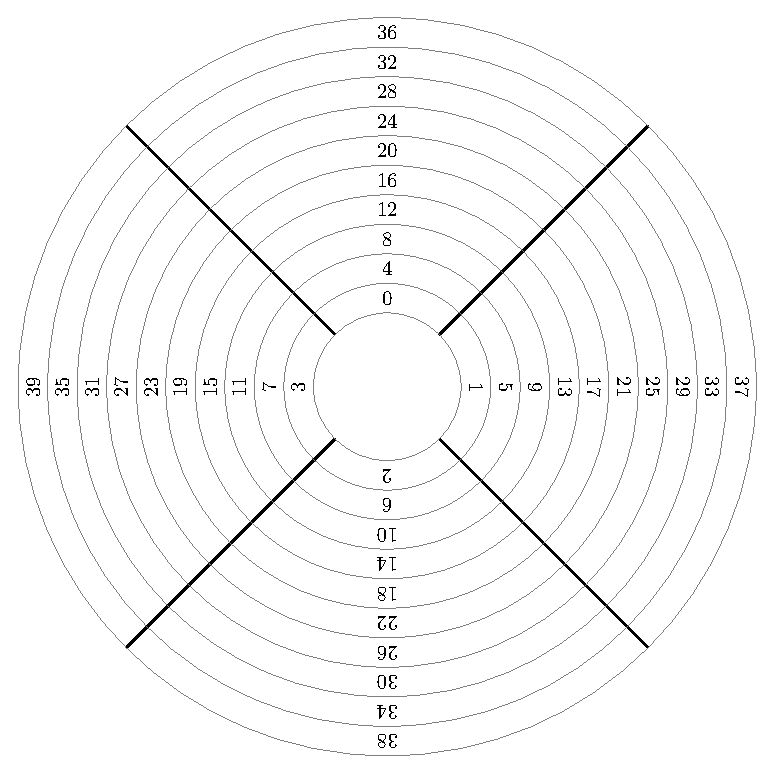
\includegraphics[width=0.7\linewidth]{tikz-wheel-modulo-4}
\caption{\textbf{Modular Arithmetic: Number Wheel Modulo $4$.}
\label{fig:modulo:wheel}}
\end{figure}


\end{document}
